\section{Performance analysis}
The performance analysis was conducted in the setting of the spiral galaxy simulation on a computer equipped with an Intel Core i7-9750H CPU (2.60GHz) and an NVIDIA GeForce GTX 1650 GPU.
By that, we mean that not only the particle distribution was the same as in \autoref{sec:spiral-galaxy-sim}, but also the configuration of the algorithms remained unchanged.
Moreover, to obtain results that most closely correspond to a real scenario of using the program, diagnostic information collection was enabled, and the simulation state was saved after each frame.
The diagnostic information mentioned here refers collectively to energy (kinetic, potential, and total), momentum, and angular momentum.
It is essential to keep in mind that in the case of the PM and \PThreeM{} methods, recording these quantities comes with an additional overhead of converting the state of the system from code to ``original'' units.
Potentially, suitable code units could also be introduced in the case of the Barnes-Hut algorithm, but we did not find this necessary.
Saving the state of the system in each frame also incurs additional overhead related to disk I/O operations.
In our implementation, the output is buffered so that data is written to disk at a reasonable frequency.
We also note that the reported running time is averaged over 100 iterations.

\begin{figure}[!ht]
    \centering
    \begin{subfigure}[b]{0.48\textwidth}
        \centering
        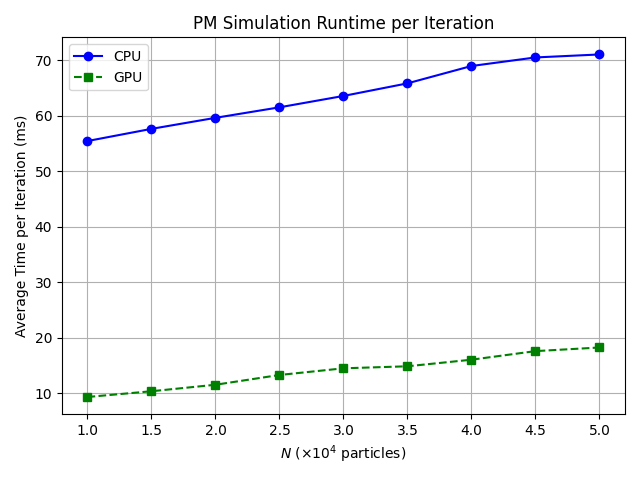
\includegraphics[width=\linewidth]{chapters/results/img/perf/pm_time.png}
        \caption{PM method}
        \label{fig:pm-running-time}
    \end{subfigure}
    \hfill
    \begin{subfigure}[b]{0.48\textwidth}
        \centering
        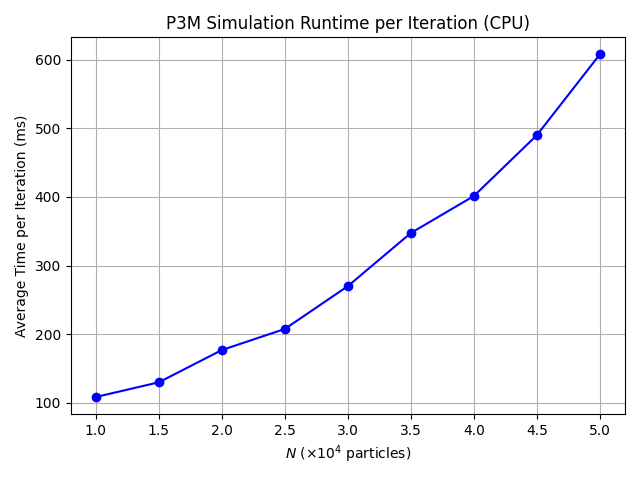
\includegraphics[width=\linewidth]{chapters/results/img/perf/p3m_time.png}
        \caption{\PThreeM{} method}
        \label{fig:p3m-running-time}
    \end{subfigure}

    \vspace{1em}

    \begin{subfigure}[b]{0.48\textwidth}
        \centering
        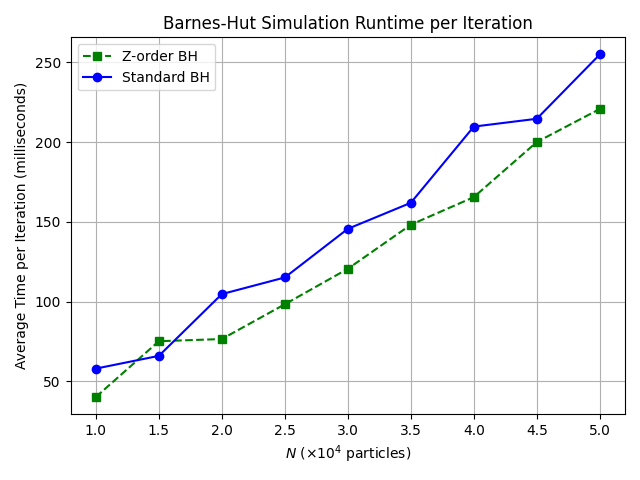
\includegraphics[width=\linewidth]{chapters/results/img/perf/bh_time.png}
        \caption{Barnes-Hut algorithm}
        \label{fig:bh-running-time}
    \end{subfigure}

    \caption{Running time of the different methods as a function of the number of particles.}
    \label{fig:method-running-time-comparison}
\end{figure}

The running time for the PM method is shown in \autoref{fig:method-running-time-comparison}.
The GPU implementation provides, at best, a five-fold speedup over the CPU implementation.
This is in stark contrast with the results reported in \autoref{subsec:gpu-variant} (1200\% speedup).
The difference between the two results stems from the fact in \autoref{subsec:gpu-variant}, we considered an ``idealized scenario'' where the data transfers from device to host and disk I/O operations were reduced to the absolute minimum, saving only the \textit{final state} of the simulation.
Both plots (GPU and CPU variants) exhibit linear time dependence as expected.

The \PThreeM{} method comes out as the least performant method among these considered in the thesis.
The runtime per iteration was up to 8.5 times longer than the CPU variant of the PM method and up to 3.5 times longer than the Barnes-Hut algorithm in its standard variant.
Moreover, it is apparent that the algorithm does not scale linearly but, we pointed out in \autoref{subsec:p3m-error-analysis}, the influence of the $O(N^2)$ direct summation part of the algorithm can reduced at the expense of weaker accuracy.

The Barnes-Hut algorithm was timed in two configurations: with the standard tree construction and the improved one (introduced in \autoref{sec:accelerating-tree-construction}).
The range of $ N $ considered in the test is too small to reveal the linearithmic runtime dependence on $N$ fully.
In any case, the Barnes-Hut algorithm comes second in the comparison, with running times 3.5 slower than the PM method in the standard variant and only 3.2 times slower if the improved tree construction is used.
We note that a comparison with \autoref{fig:z-order-tree-time} reveals that the tree construction is responsible for around 15\% of the total running time of the simulation.